\chapter{Semantic Bespin: a Semantic RESTful Mashup}

\section{Introduction}

In previous chapters we have specified a theoretical model for semantic RESTful web services, we have build a technical
specification of the model and we have built software libraries, Siesta and Semantic REST, for enabling semantic RESTful web services in the
server and client sides of a web application.\\ 

In this chapter we will introduce Semantic Bespin, a web application that
consumes different web services from a Javascript client, a kind of web application usually known as mashup.
The client side of the application as well as the implementation of the services are built on top of the Siesta
Javascript framework for Javascript and the Semantic REST Ruby library that were introduced in previous chapters.\\

This application pretends to be a sample of the kind of web applications that can be achieved through the use of
semantic RESTful web services, and also as an use case for the Siesta and Semantic REST libraries.

\section{Description of the Application}

The main goal of Semantic Bespin is offering an Integrated Development Environment (IDE) allowing geographically distributed
teams of people work together in software projects using a single tool running inside the web browser.\\

The main features that Semantic Bespin offers to developers are summarized in the following points:

\begin{itemize}
\item Code editor and file browser
\item Remote storage and management of the project configuration 
\item Source code management supporting the Git (\url{www.git-scm.org/}) source version control system
\item Mechanism for notifications and communications between developers.
\end{itemize}

As we have mentioned, the application is not a monolithic one, it is the result of mixing different services exposing
its resources as semantic meta data. The table \ref{services_table_1} shows the services used and which functionality
they provide:

\begin{table}
\begin{tabular}{|l|l|}
  \hline
  \multicolumn{2}{|c|}{Services used in Semantic Bespin} \\
  \hline
  Service & Functionality \\
  \hline
  Bespin & code edition \\
  Rails Bespin back end & project management \\
  XINGhub & Git repository support \\
  Twitter & notifications \\
  \hline
\end{tabular}
\caption{Main services used in the Semantic Bespin application}
\end{table}

Some of these services and applications, like Bespin and XINGhub, are existent software projects whose source code was
available for its modification. It has been possible to adapt those services in order to use the Semantic REST library
for exposing its services as RESTful semantic web services.
Other services like Twitter are commercial applications whose code is not available for modification, but with a public
REST API that can be described using the external services features (\ref{desc_ext_servs}) of the Semantic REST library.
Finally, some other components like the Rails Bespin back end have been developed from scratch using the Semantic REST
library as the foundation for the services exposed in the application.\\

\subsection{Bespin}

Bespin (\url{https://bespin.mozilla.com/}) is a project from the Mozilla's Foundation Labs developing an open source code web editor. Bespin is in the
spirit of classic editors like Emacs, where a extensible programming language (Emacs Lisp in the case of Emacs,
Javascript in the case of Bespin) serves as the base of an environment where editing functions are implemented. The
behavior of the editor can be extended or modified at run time by evaluating new Javascript code in any moment.\\

Bespin has been built using the latest technologies available in the browser, making a heavy use of the canvas tag through the
Thunderhead library, also developed in the Mozilla's Foundation Labs, that provides a framework of components for
the browser canvas similar to Adobe's Flex components. The rest of the editor is built using the Dojo Framework.\\

Bespin can be obtained from the Mozilla Labs site. It already offers part of the functionality of Semantic Bespin, but
does it using ad hoc web services exposed from a Python back end. Bespin also relies in the Mercurial (\url{http://mercurial.selenic.com/wiki/}) version control
system as the basis of its SCM features.\\

The source code from Mozilla has been modified in several ways adapting it to the Siesta Javascript framework and
the Semantic REST library. The following points summarize the most important modifications:

\begin{itemize}
\item The Python back end has been substituted by a new Rails back end RESTful semantic web services exposed through
  the Semantic REST library.
\item Server communication functions in the client have been replaced by Siesta Framework objects.
\item The support for Mercurial has been replaced by Git through the use of XINGhub back end RESTful semantic web services.
\item The original support for messages between users have been replaced by a Twitter status service whose description
  is exposed in the Bespin Rails back end.
\item Additional functionality and graphical interface elements have been added to support the exploration of the client
  triplets repository and other required changes in components like the file browser.
\end{itemize}

\subsection{XINGhub}

XINGhub is a software project developed by the company XING AG as a tool for social coding: mixing social features like
the following of users or the exchange of messages with the regular features of a source control tool, the hosting of
source repositories. It has been modeled after the Github (\url{http://github.com}) commercial service.\\

XINGhub does not offer a services API so the source code had to be modified to export part of its model layer as a set
of RESTful semantic services with the Semantic REST library that could be consumed from the Semantic Bespin Javascript
client:

\begin{itemize}
\item A public key service have been created that allows a client to upload a public SSH key. This is required for it to
  retrieve and modified the remote repository of code.
\item A Repository service have been created that allows a client to create repositories of code hosted in XINGhub.
\end{itemize}

\subsection{Twitter}

Twitter (\url{http://twitter.com}) is web service allowing users to exchange small messages of 140 characters. It offers a REST API with services
for updating messages, retrieving all the messages of an user, etc.\\
A description of the status services of Twitter has been added to the Bespin Rails back end in order for the Semantic
Bespin client to consume Twitter's API.

\section{Architectural Overview}

The figure \ref{bespin_arch_1} shows the main resources in the Semantic Bespin application independently of the location
of the services.

\begin{table}{h!}
\noindent\makebox[\textwidth]{%
\begin{tabularx}{1.4\textwidth}{XX}
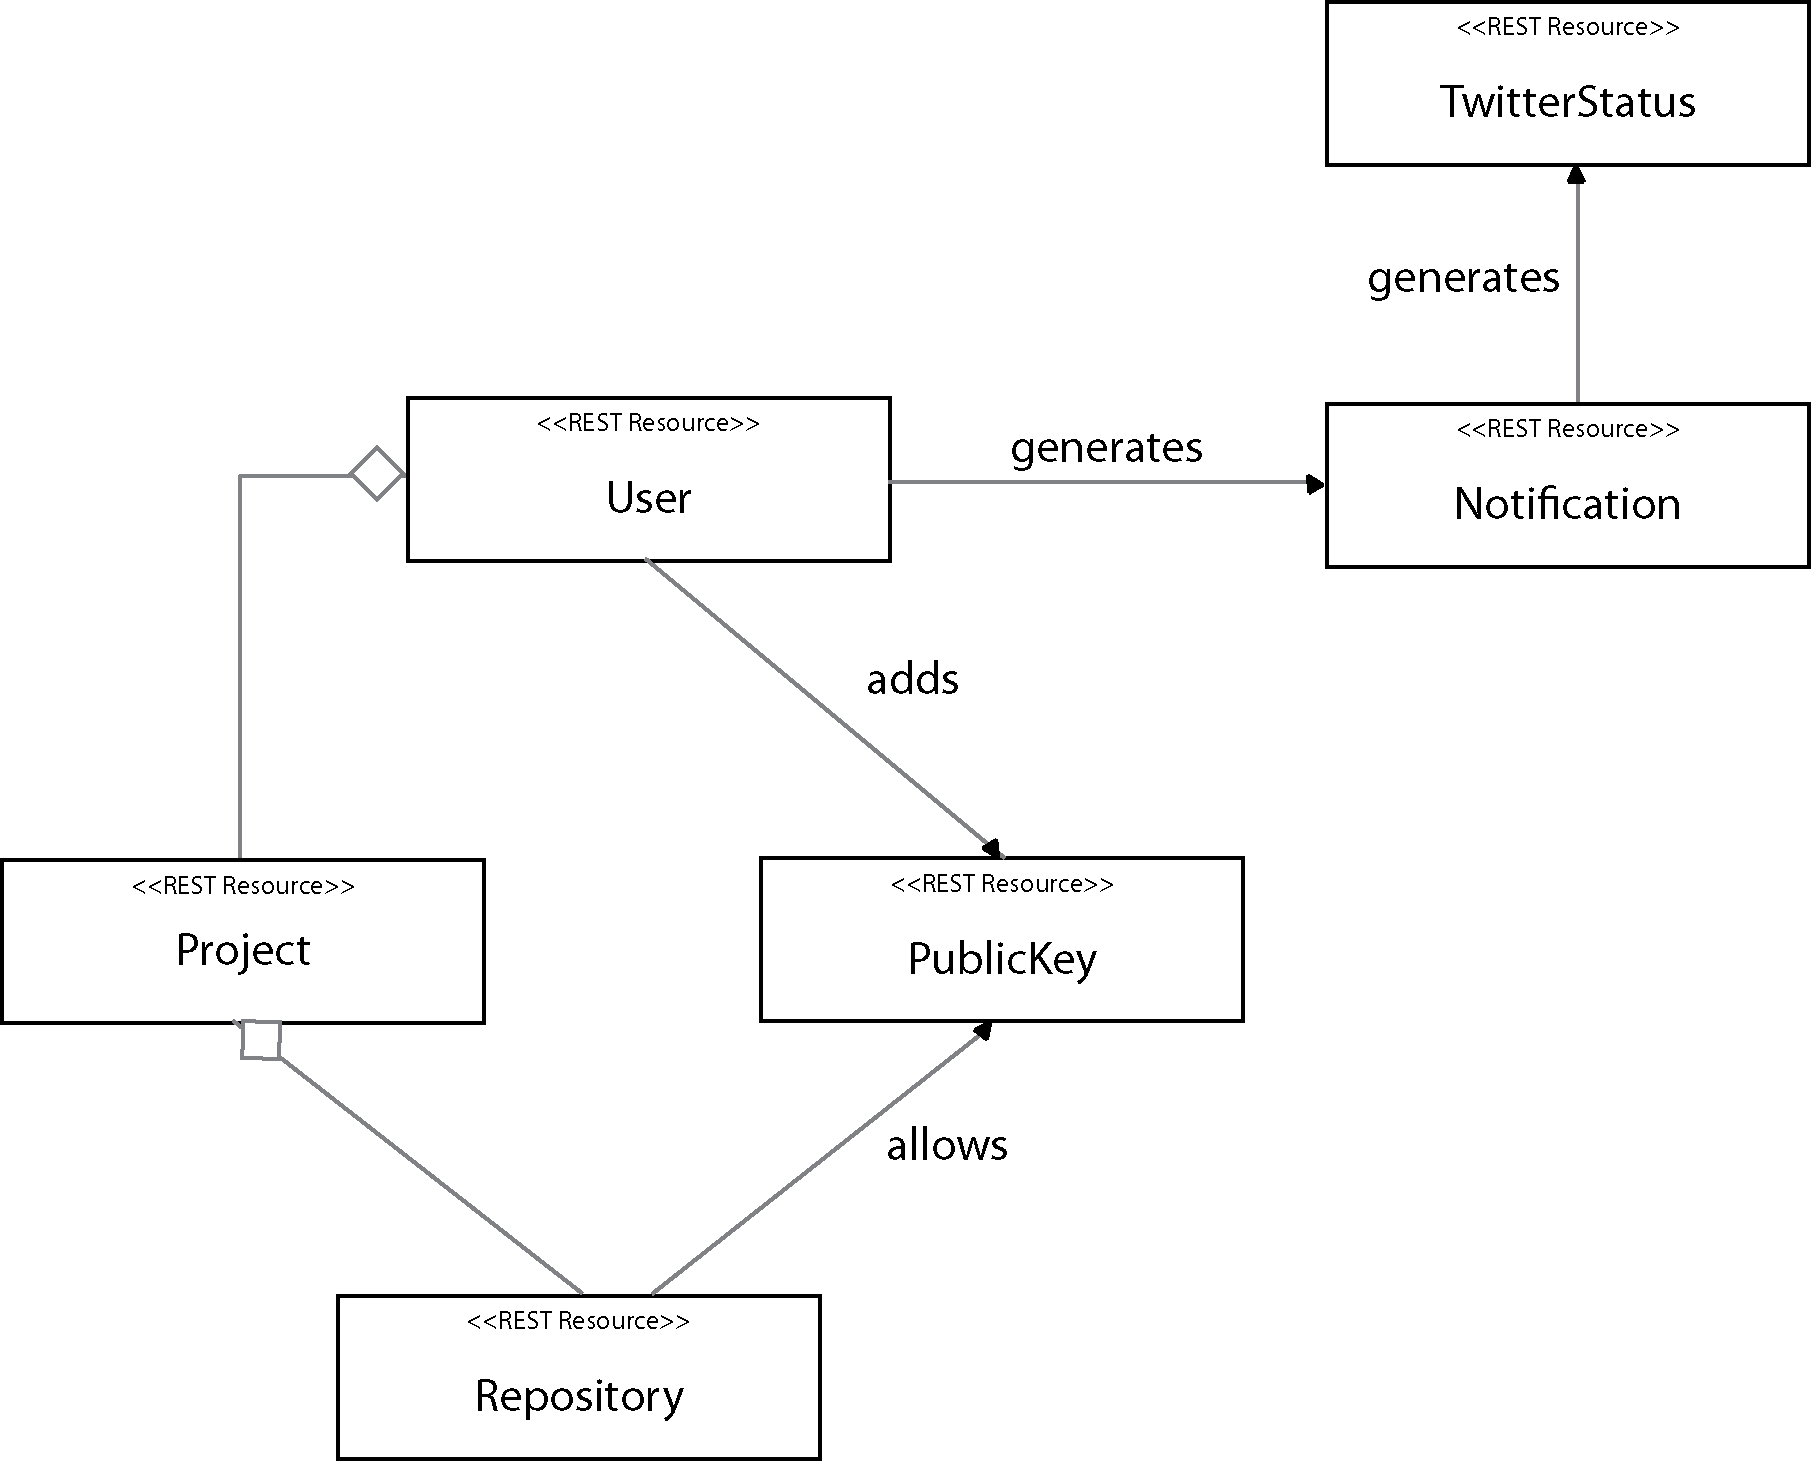
\includegraphics{applicationResources.png}
\end{tabularx}}
\caption{Main resources in the Semantic Bespin application}
\label{bespin_arch_1}
\end{table}

The set of services of the application are consumed from the Semantic Bespin Javascript from different locations and
with different purposes. The next table summarizes where are the services located and why they are consumed.

 \begin{table}
\begin{tabular}{|l|l|l|l|}
  \hline
  \multicolumn{3}{|c|}{Services used in Semantic Bespin} \\
  \hline
  Service & Method & Location & Purpose \\
  \hline
  User& POST & Rails Bespin&  Registration of a user\\
  User& GET & Rails Bespin & Login of a user\\
  Project& POST & Rails Bespin & Creation of a new project\\
  Project& GET & Rails Bespin & Retrieval of the information of a project\\
  PublicKey& POST & XINGhub & Allows access to a repository to a new\\
                 &        &                                    & public SSH key\\
  PublicKey& GET & Rails Bespin & Retrieves the public key of the \\
                 &        &                                    & Rails Bespin back end machine \\
  Repository& POST & XINGhub &Creates a new repository\\
  Repository& GET & XINGhub & Retrieves the data of one repository\\
  TwitterStatus& PUT & Twitter(Proxy) & updates the status of a Twitter user\\
  TwitterStatus& GET & Twitter & retrieves the status of a Twitter user\\
  \hline
\end{tabular}
\caption{Location of the services of the Semantic Bespin application}
\end{table}

The figure \ref{bespin_arch_2}  shows how these services are deployed across the different services.

\begin{table}{h!}
\noindent\makebox[\textwidth]{%
\begin{tabularx}{1.4\textwidth}{XX}
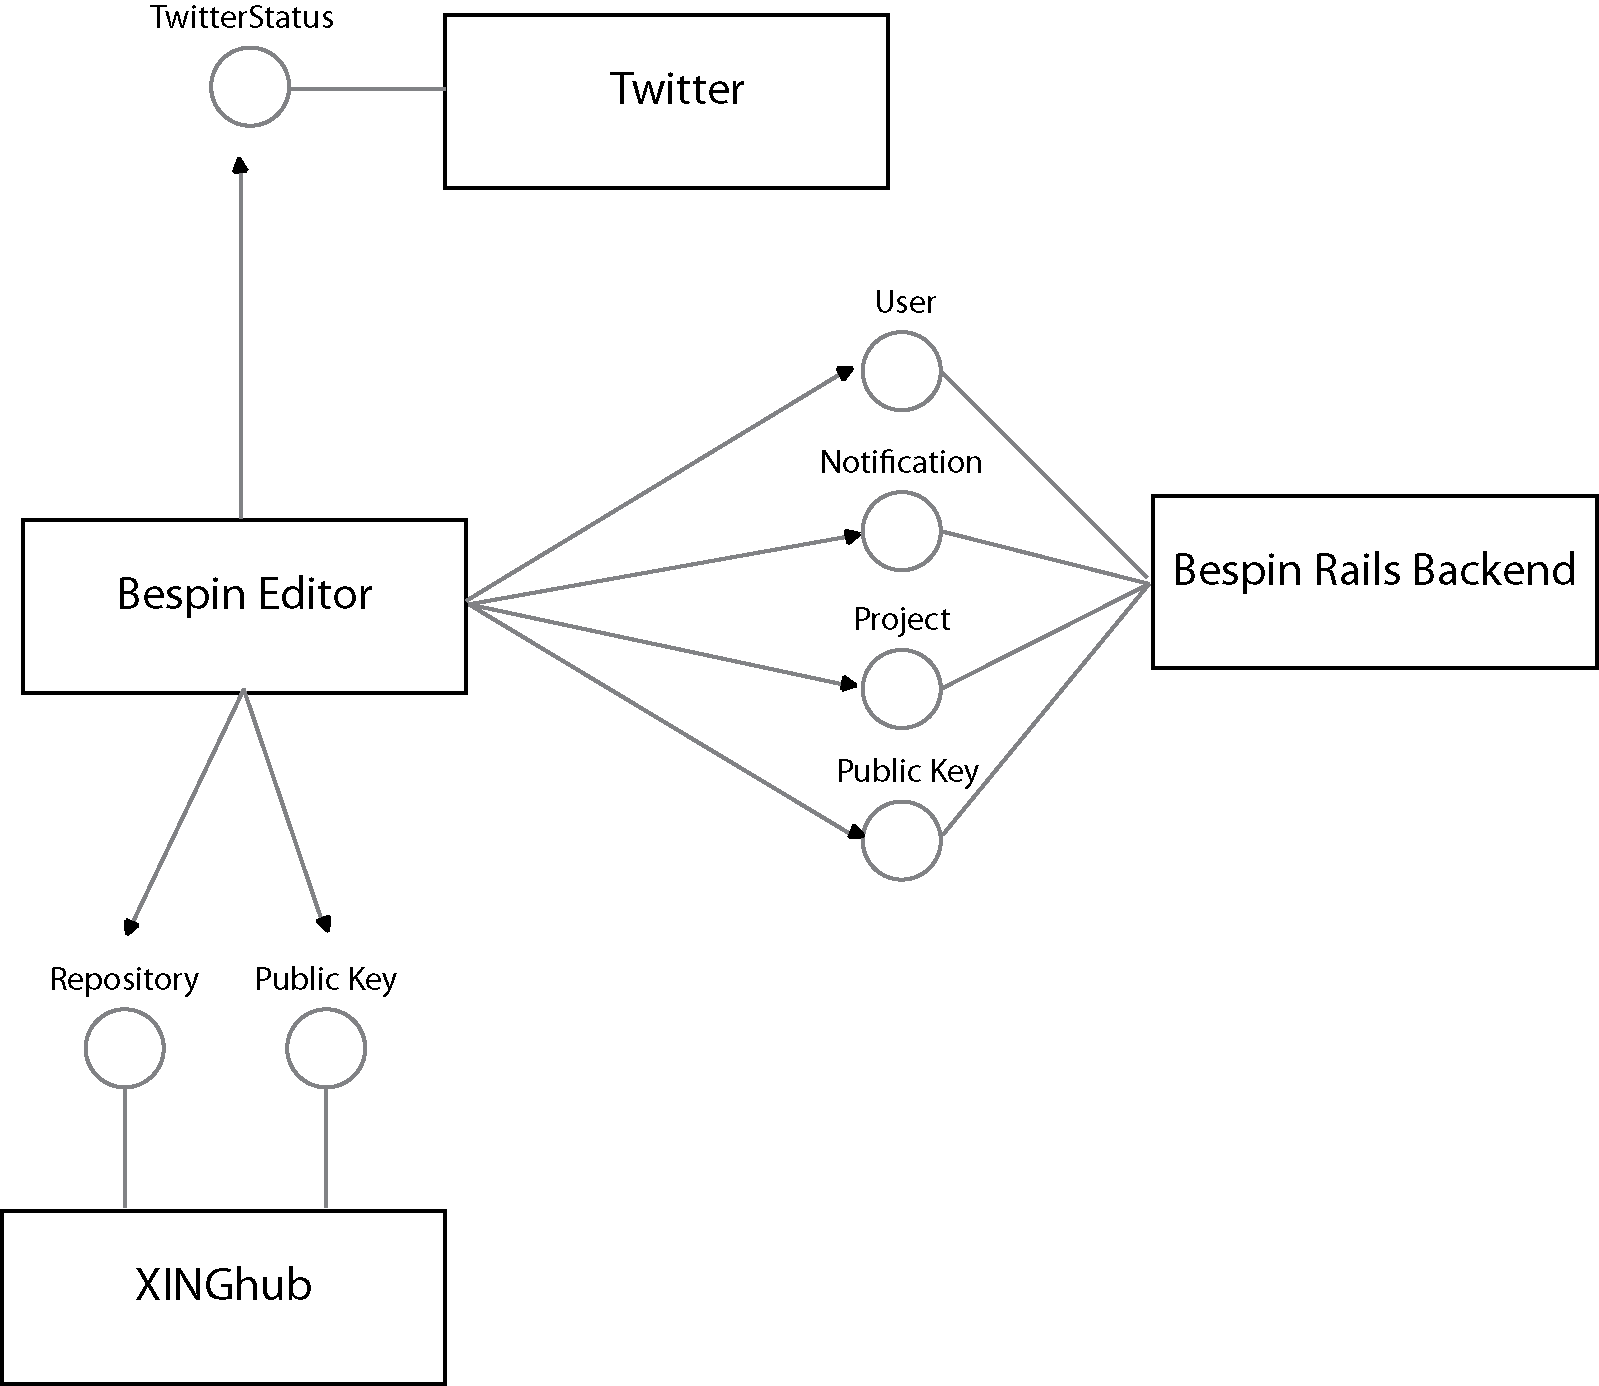
\includegraphics{loc_servs.png}
\end{tabularx}}
\caption{Main resources in the Semantic Bespin application}
\label{bespin_arch_2}
\end{table}

\subsection{User resource}

The \texttt{User} resource is exposed by the \texttt{UserService} in the Bespin Rails back end. It is defined by a User
Ruby on Rails model with some annotations for exporting the model as a RESTful semantic web service. the code in
\ref{bespin_user_1} shows how the resource is defined

\begin{table}
\vspace{5 mm}
\begin{lstlisting}
require 'semantic_resource/base'

class User < ActiveRecord::Base
  

  has_many :current_files
  has_many :projects

  # Semantic definition
  include SemanticResource

  set_resource_namespace :sb, "http://semantic_bespin.org"

  set_resource_mapping do |resource|
    resource[:xinghub_login] = {:uri => "http://xinghub.com#login" }
    resource[:username] = {:uri => [:sb,"#username"] }
    resource[:password] = {:uri => [:sb,"#password"]}
    resource[:email] = {:uri => [:sb,"#email"] }
    resource[:twitter_login] = {:uri => [:sb,"#twitter_login"] }
 end

  define_show_operation(:controller => 'users',
                        :action => 'show',
                        :url_parameters => [:username,:password],
                        :show_id => false)

  define_create_operation(:controller => 'users',
                          :action => 'create')

  def find_project_by_name(project_name)
    projects.find(:first, :conditions => { :short_name => project_name})
  end
end
\end{lstlisting} 
\vspace{5 mm}
\caption{User resource definition}
\label{bespin_user_1}
\end{table}

We can see how the properties of the model contains information about the user username and password as well as
information about its usernames in the XINGhub and twitter service.\\

The \texttt{User} service is later consumed from the semantic bespin client using the Siesta Framework as its shown in
the listing \ref{bespin_user_2}

\begin{table}
\vspace{5 mm}
\begin{lstlisting}
SemanticBespin.User = new Siesta.Model.Class({
  schemaUri: "http://localhost:3000/schemas/models/User",
  serviceUri:"http://localhost:3000/schemas/services/UserService",
  getOperationUri: "http://localhost:3000/schemas/services/User#showUser",
  postOperationUri: "http://localhost:3000/schemas/services/User#createUse"
});

SemanticBespin.User.definePropertiesAliases({
   id:"http://semantic_rest/siesta#id",
   xinghubLogin: "http://xinghub.com#login",
   username: "http://semantic_bespin.org#username",
   password: "http://semantic_bespin.org#password",
   email: "http://semantic_bespin.org#email"
   twitter_loginl: "http://semantic_bespin.org#twitter_login"
});
\end{lstlisting} 
\vspace{5 mm}
\caption{Consuming the User service}
\label{bespin_user_2}
\end{table}

\subsection{Project resource}

The \texttt{Project} resource is exposed by the \texttt{ProjectService} in the Semantic Rails back end. It stores
information about the Project, identified by a name, a repository URL and a Twitter user and password. The repository
URL is the URL of a XINGhub repository, the Twitter credential will be used to send notification that can be received by
all the users working in the project.\\

The code at \ref{bespin_prj_1} shows the definition of the service:

\begin{table}
\vspace{5 mm}
\begin{lstlisting}
require 'semantic_resource/base'

class Project < ActiveRecord::Base

  # Semantic definition
  include SemanticResource

  set_resource_namespace :sb, "http://semantic_bespin.org"

  set_resource_mapping do |resource|
    resource[:short_name] = {:uri => [:sb,"#shortname"] }
    resource[:repository_url] = {:uri => [:sb,"#linkedToRepository"] }
    resource[:twitter_user] = {:uri => [:sb,"#twitter_user"] }
    resource[:twitter_password] = {:uri => [:sb,"#twitter_password"] }
  end

   define_show_operation(:controller => 'projects',
                         :action => 'show',
                         :url_parameters => [:username,:password],
                         :input_messages => { User => [:username, :password]})

  define_index_operation(:controller => 'projects',
                        :action => 'index',
                        :url_parameters => [:username,:password],
                        :input_messages => { User => [:username, :password]})

   define_create_operation(:controller => 'projects',
                         :action => 'create',
                         :url_parameters => [:username,:password],
                         :input_messages => { User => [:username, :password]})

  ...
end

\end{lstlisting} 
\vspace{5 mm}
\caption{Consuming the User service}
\label{bespin_prj_1}
\end{table}

In the definition of the service, besides the \texttt{Project} triple graph, an additional input message for the operations have
been added with the triple graphs of an \texttt{User}. The listing at \ref{bespin_prj_serv_1} shows a portion of the
generated RDF graph corresponding to the GET operation of the service. The presence of the additional message can be
observed.

\begin{table}
\vspace{5 mm}
\begin{lstlisting}
<http://localhost:3000/schemas/services/Project#showProject> <http://www.w3.org/1999/02/22-rdf-syntax-ns#type> wsl:Operation ;
  rdfs:label "retrieves Project resource with id {id}" ;
  hr:hasMethod  "GET" ;
  hr:hasAddress "http://localhost:3000/projects/show/{id}?password={password}&username={username}"^^<hr:URITemplate> ;
  wsl:hasInputMessage [
    <http://www.w3.org/1999/02/22-rdf-syntax-ns#type> wsl:Message ;
    sawsdl:modelReference <http://localhost:3000/schemas/models/Project> ;
    sawsdl:loweringSchemaMapping <http://localhost:3000/schemas/lowering/Project/show.sparql>
  ] ;
  wsl:hasInputMessage [
    <http://www.w3.org/1999/02/22-rdf-syntax-ns#type> wsl:Message ;
    sawsdl:modelReference <http://localhost:3000/schemas/models/User> ; 
    sawsdl:loweringSchemaMapping <http://localhost:3000/schemas/lowering/Project/show/User.sparql>
  ] ;
  hr:hasInputParameter [
    <http://www.w3.org/1999/02/22-rdf-syntax-ns#type> hrjs:JSONPCallback ;
    hr:parameterName "callback"
  ] ;
  wsl:hasOutputMessage [
    <http://www.w3.org/1999/02/22-rdf-syntax-ns#type> wsl:Message ;
    sawsdl:modelReference <http://localhost:3000/schemas/models/Project>  ] .
\end{lstlisting} 
\vspace{5 mm}
\caption{The GET opertion of the Project Service}
\label{bespin_prj_serv_1}
\end{table}

In the Semantic Bespin Javascript client this service is consumed for instance when creating a new project. The figure
\ref{bespin_new_dialog} show the user interface for the creation of a new project, and the listing at
\ref{bespin_new_src} shows a portion of the callback function for that dialog that invokes the POST operation of the
\texttt{ProjectService}.

\begin{table}{h!}
\noindent\makebox[\textwidth]{%
\begin{tabularx}{1.2\textwidth}{XX}
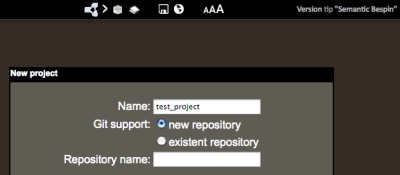
\includegraphics{new_dialog.png}
\end{tabularx}}
\caption{Semantic Bespin new Project dialog}
\label{bespin_new_dialog}
\end{table}

\begin{table}
\vspace{5 mm}
\begin{lstlisting}
var project = SemanticBespin.Project.build({
    shortname: prjName,
    linked_to_repository: cloneUrl,
    twitter_user: twitterUser,
    twitter_password: twitterPassword
});
project.addInputMessage(_currentUser.toGraph());
project.save(function(savedProject) {                            
   SemanticBespin.addToRegistry(savedProject.uri, "projects", "created", savedProject);
   theProject = {name:savedProject.get('shortname'), 
                        instance:savedProject}
   bespin.publish("project:created",theProject);

   dojo.style(form,"display","none");
});
\end{lstlisting} 
\vspace{5 mm}
\caption{Consuming the Project service}
\label{bespin_new_src}
\end{table}

\subsection{PublicKey resource}

The \texttt{PublicKey} resource is exposed by the Bespin Rails back end and by XINGhub. The Rails back end allows the GET
operation on the service so the clients can retrieve the public key of the back end. XINGhub exposes the service with
the POST operation. This operation can be used by clients for allowing users to grant access to a repository to requests
authentified by that public key.\\
The Javascript client, when creating a new project linked to a XINGhub repository retrieves the public key of the Bespin
Rails back end and consumes the XINGhub POST \texttt{PublicKey} service to allow access to the repository to the Bespin Rails back
end. When the Bespin Rails back end receives a \texttt{Project} service POST request from the client, tries to clone the remote
repository with its public key.\\
The whole process is represented in the diagram \ref{besping_public_key}


\begin{table}{h!}
\noindent\makebox[\textwidth]{%
\begin{tabularx}{1.4\textwidth}{XX}
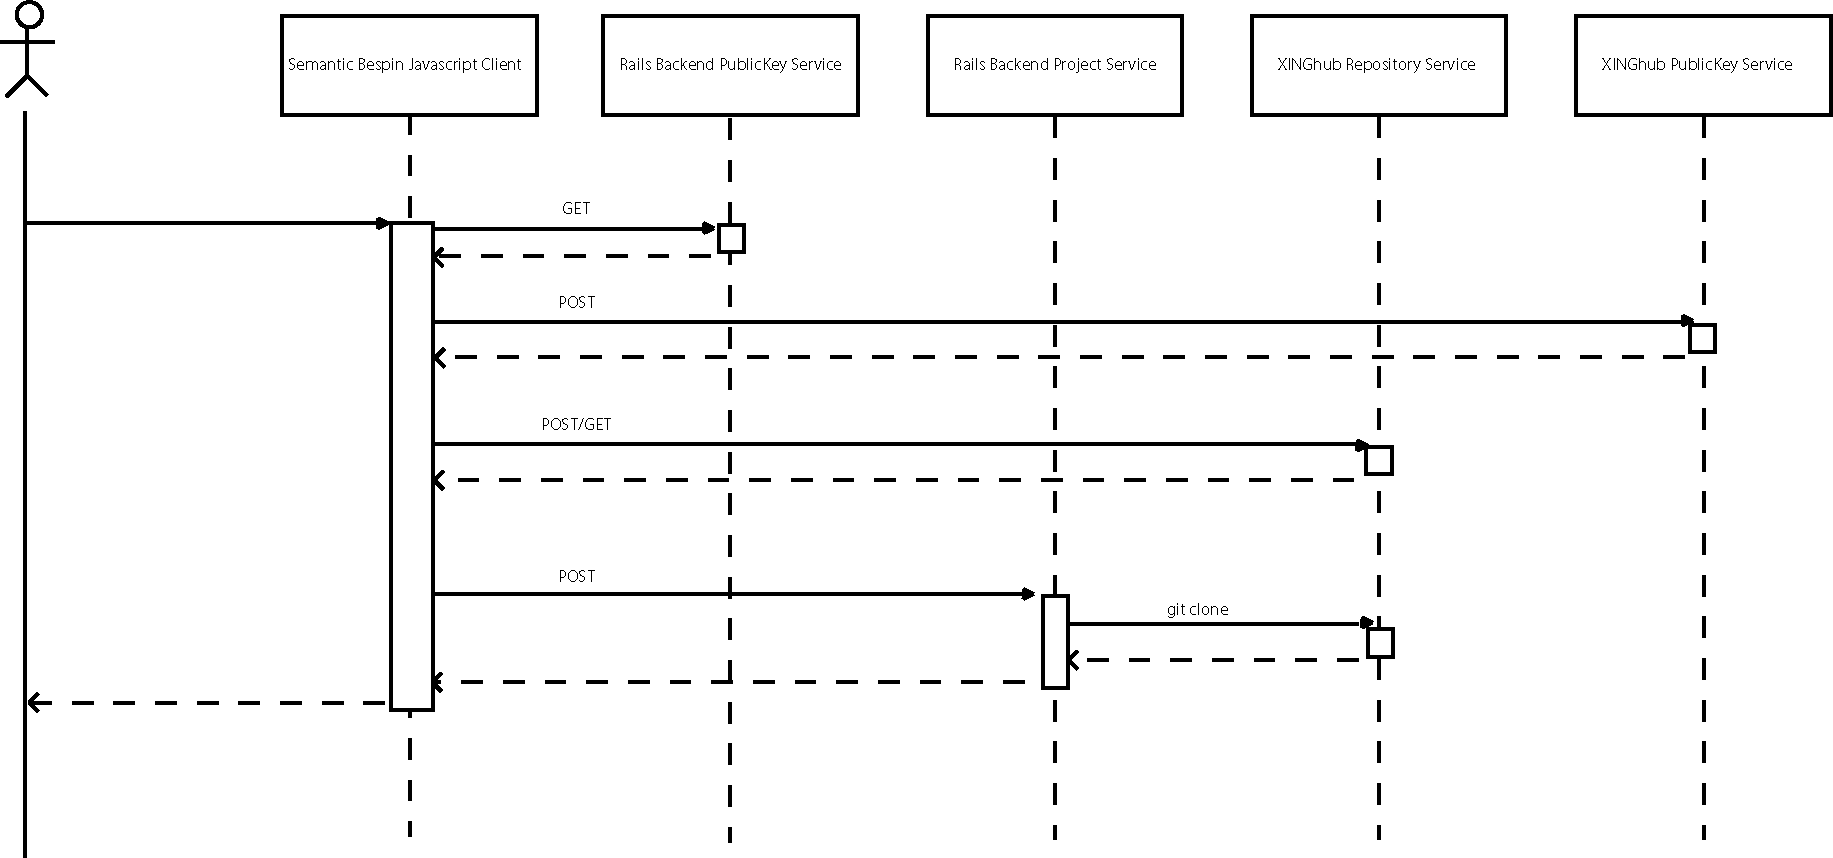
\includegraphics{public_key.png}
\end{tabularx}}
\caption{Creation of a new project exchanging public keys}
\label{bespin_public_key}
\end{table}


\subsection{Repository resource}

The \texttt{Repository} resource and service are located into the XINGhub application. They are extensions to the
\texttt{Repository} model of the application and the service is tailored into the \texttt{Repository} controller of the
application.\\

The main methods of the \texttt{RepositoryService} are the methods GET and POST. With a GET request the data for
a repository, including its URI,  can be retrieved from the name of the repository. With a POST request a new repository
is created. Those two methods are used by the Semantic Bespin client to link an existent or new repository to a
client.\\

XINGhub stores in its database the data of the new repository and spawns a request to a worker process that
asynchronously issues the actual Git commands for the creation of the Git repository. This commands are executed providing the public SSH key
associated to the user, so the privileges check is done by the Git application. If the creation of the repository is
successful, the worker process updates the data base state information associated to the repository.\\

The code listing at \ref{bespin_repository_serv_1} shows the code containing the description of the service.


\begin{table}
\vspace{5 mm}
\begin{lstlisting}
  set_resource_namespace :xh, "http://xinghub.com"

  set_resource_mapping do |resource|
    resource[:name] = {:uri => [:xh,"#repository_name"] }
    resource[:url] = {:uri => [:xh,"#repository_url"] }
    resource[:uid] = {:uri => [:xh,"#repository_uid"] }
  end

  define_show_operation(:controller => 'repositories',
                        :action => 'show',
                        :url_parameters => [:url],
                        :show_id => false)

  define_create_operation(:controller => 'repositories',
                          :action => 'create',
                          :url_parameters => [:login],
                          :input_messages => { User => [:login]})
\end{lstlisting} 
\vspace{5 mm}
\caption{Definition of the Repository resource}
\label{bespin_repository_serv_1}
\end{table}


\subsection{TwitterStatus service}
The \texttt{TwitterStatusService}  is a wrapper around the status service of the Twitter API. Two methods of the Twitter API are
used in Semantic Bespin: \texttt{statuses/show} and \texttt{statuses/update}. \texttt{statuses/show} recovers the
current status of a Twitter user, \texttt{statuses/update} allows a user to update such an status.\\
In the Semantic Bespin application, each Semantic Bespin project can have an associated Twitter user and password. A
Semantic Bespin user can also have a property stating its twitter user name. When the Javascript client generates some
kind of notification, for instance, a user has started editing a file, the client consumes Twitter's
\texttt{statuses/update} method through the \texttt{TwitterStatusService} description. As a result, the status of the
Twitter user identified by the login and password of the Semantic Bespin project is updated. The status message contains
the text of the notification and the Semantic Bespin user's Twitter user name as the originator of the notification.\\

The Semantic Bespin client also polls with a certain frequency the \texttt{statuses/show} Twitter's API method in order
get the notifications originated by others users.\\

The listing \ref{bespin_twitter_yaml} shows the YAML description of the Twitter service as it is stored in the Rails
Bespin back end. This YAML description is transformed by the Semantic REST library into a RDF Graph describing how to
consume the Twitter API according to the hRESTS specification.\\


\begin{table}
\vspace{5 mm}
\begin{lstlisting}
service:

  identifier: twitter
  label: A Twitter service description
  model: http://localhost:3000/twitter_proxy/status

  operations:
    - identifier: twitter#showStatus
      label: show status
      method: GET
      address: http://twitter.com/statuses/user_timeline.json?screen_name={twitter_user}&count=1

      input_messages:

        - name: twitter_user
          description: Identifier of the user assigned to the project
          model: http://localhost:3000/schemas/models/Project
          lowering: http://localhost:3000/twitter_proxy/show_status_lowering_user.sparql

      input_parameters:

      - type: JSONPCallback
        parameterName: callback
        description: The name of the callback function to be invoked by the server

      output_messages:

      - name: theStatus
        description: The JSON description of the status
        model: http://localhost:3000/twitter_proxy/status
        lifting: http://localhost:3000/twitter_proxy/status_lifting.js
\end{lstlisting} 
\vspace{5 mm}
\caption{Semantic Bespin Twitter Service YAML description}
\label{bespin_twitter_yaml}
\end{table}

\begin{table}
\vspace{5 mm}
\begin{lstlisting}
    - identifier: twitter#updateStatus
      label: update the status
      method: POST
      address: http://localhost:3000/notifications/update?status={text}&username={username}&password={password}
      
      input_messages:
      
      - name: theUser
        description: The user whose status is going to be updated
        model: http://localhost:3000/schemas/models/Project
        lowering: http://localhost:3000/twitter_proxy/put_status_lowering_user.sparql

      - name: theStatus
        description: The new status
        model: http://localhost:3000/twitter_proxy/status
        lowering: http://localhost:3000/twitter_proxy/put_status_lowering.sparql

      output_messages:

      - name: theUpdatedStatus
        description: The JSON description of the status
        model: http://localhost:3000/twitter_proxy/status
        lifting: http://localhost:3000/twitter_proxy/status_lifting.js
\end{lstlisting} 
\vspace{5 mm}
\caption{Semantic Bespin Twitter Service YAML description (cont)}
\label{bespin_twitter_yam_2}
\end{table}

The \texttt{statuses/update} method of the Twitter API requires the client to authenticate itself using HTTP Basic
Authentication. This kind of authentication requires the client to send HTTP headers with its user name and
password. Unfortunately this headers cannot be sent through a JSONP request and a AJAX request is neither possible for
a client outside the Twitter domain, due to the security model of the web browser. This makes impossible for the
Semantic Bespin Javascript client to consume directly the \texttt{statuses/update} API service. To solve this issue this
requests are sent to a Rails Bespin back end service that acts as proxy for the client to the Twitter API.\\

The code listing at \ref{bespin_client_twitter} shows how the Javascript client polls periodically the Twitter
\texttt{statuses/show} service to retrieve new notifications from others users.


\begin{table}
\vspace{5 mm}
\begin{lstlisting}
SemanticBespin.projectStatusPoller = function() {
    setTimeout(function() {
            
            if(SemanticBespin.currentProject != null) {
               var status = SemanticBespin.TwitterStatus.build({ });
                status.addInputMessage(SemanticBespin.currentProject.toGraph());
                SemanticBespin.TwitterStatus.find(status,function(retrievedStatus) {
                        var txt = retrievedStatus.get("text");
                        if(txt != SemanticBespin.projectStatusLast) {
                            SemanticBespin.projectStatusLast = txt;
                            SemanticBespin.pushNotification(txt, retrievedStatus.get("createdAt"));
                        }
                });
            } 
            SemanticBespin.projectStatusPoller();            
        }, 10000);
};
\end{lstlisting} 
\vspace{5 mm}
\caption{Consuming the Project service}
\label{bespin_client_twitter}
\end{table}

\section{Conclusions}
The building of the Semantic Bespin application has been useful as an example of what can be achieved with the use
semantic technologies and REST architectures in the development of web applications, specially when they consist of the
mixing of several pre existent applications or services.\\

It has also served as a test for the RESTful semantic web services libraries built, the Siesta Framework and the
Semantic REST library, it has also pointed the features missing in these libraries and how they could evolve and
improve.\\

Apart from that, the most inmediate benefit of the use of semantic standards for the description of RESTful web services
through the use of the Semantic REST and Siesta libraries has been the increase in productivity achieved. Many tasks
needed in the building and consumption of a web services such as the marshalling and unmarshalling of data, network
communications, etc. have been automated with the use of these libraries.\\

The chances for the exchange and the access to data increase notably due to the presence of an additional meta data
layer. This makes possible to automate the access to data that were not originally designed to be used outside the
application where they are stored.\\

The Open World semantics present in Description Logics and also present in the semantic standards is specially useful for
the description of web resources. It allows to build gradually the resources adding assertions retrieved from different
services. \\

The development of the Semantic Bespin application has also served as good example of the different ways to use the
Semantic REST library. It has been used to describe new resources from scratch in the Rails Bespin back end, to adapt
existent services in the case of XINGhub or to wrap third party services as it has been the case of Twitter.\\

Nevertheless, some aspects of the development of web applications cannot be easily modeled as REST resources. Such is
the case of authentication. This suppose a serious issue when adapting external services as it has been the case of
Twitter. This problem is specially serious due to the lack of support of authentication standards that could be used across different
services and applications such as OpenId or OAuth.\\

It has also been interesting how the use of onthologies allows to hide the heterogeneous origin of the data consumed in
the client. As an example the client does not need to know if the data of \texttt{PublicKey} comes from the Rails Bespin
back end or XINGhub because both data are described using the same onthology. In this way it would e easy to allow the
interaction with different control version systems besides Git like Mercurial or Darcs, as long as its data could be
mapped to the same onthology. At the end the effective decoupling of client and servers can be obtained more effectively
through a careful design of the semantic layer or the use of standard onthologies.\\
It is also interesting how the use of this kind of architectures allows the creation of rich internet applications, with
similar features to desktop applications, preserving a RESTful layer in the back end the is true to the principles of the
HTTP protocol and adding an extra layer of semantic data.